\chapter{Audit Outcomes}

% Note: Since we don't have access to true labels of original test set of the Kaggle Competition, we split the original training data into train and test data (4:1 ratio) for validating the model performance across various audit tests. The results we obtained may or may not be highly accurate, since train-test split might have caused information leakage. \\
% (maybe try to generate dp synthetic dataset using the "final depression dataset" in correlated mode to once check the model performance generalization???) 



% 1. dropping name and city has no significant affect on accuracy of the model.\\
% 2. for 2 submodels gb and adb, numerical value columns were imputed with mean values - [Academic Pressure, Work Pressure, CGPA, Study Satisfaction,Job Satisfaction] - this seems unjustifiable, since imputing mean of academic pressure value to a professional, or work pressure value to a student doesn't make sense. Yet, when model was run for these 2 categories seperately, with dropping the non-relevant columns, the metrics obtained were quite similar to what was obtained before, implying the model's robustness, which can be explained by the usage of ensembling several models \parencite{black2021selective}. The FPR  and FNR parity genderwise ia high, however, w.r.t. employment status, working professionals have high FNR and students have high FPR. \\
% (-- have to look into 'Profession' and 'CGPA' for this. And lime values too. )\\
% checked lime values for 10 false positive classifications--pattern?\\
% top 5 points for explanations suggest ---\\


\section{Experiments}
Initial experiments showed that dropping the \texttt{Name} and \texttt{City} features from the dataset had no significant impact on the model’s overall accuracy as well as other metrics like FNR/FPR and fairness metrics as can be seen in Figure~\ref{fig:orig_vs_drop}. This suggests that these features did not carry meaningful predictive information and that the model is not overly reliant on potentially privacy-sensitive attributes. Other relevant results w.r.t. overall and genderwise FNR/FPR/Selection Rate Difference are included in Appendix~\ref{feature_corr} (Figures~\ref{fig:region_overall},~\ref{fig:region_gender}). 

\begin{figure}[H]
    \centering
    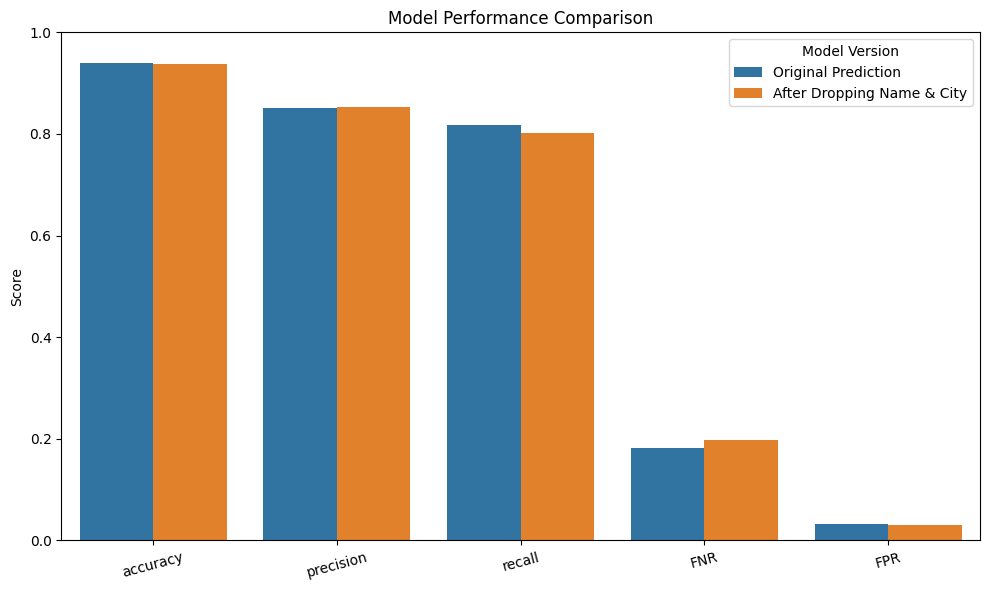
\includegraphics[width=0.6\linewidth]{figures/orig_vs_drop.png}
    \caption{Results before and after dropping sensitive features}
    \label{fig:orig_vs_drop}
\end{figure}

An interesting observation emerged from examining how the two sub-models : Gradient Boosting (GB) and AdaBoost (ADB) handled missing data. These models imputed missing values in numerical columns such as \texttt{Academic Pressure}, \texttt{Work Pressure}, \texttt{CGPA}, \texttt{Study Satisfaction}, and \texttt{Job Satisfaction} using mean imputation. While this method is common, it can be problematic in our context. For example, imputing the average academic pressure of students for a working professional lacks contextual validity, and vice versa. Yet, when the ensemble model was retrained and evaluated separately for students and working professionals (after dropping the irrelevant features for each group), the resulting performance metrics were close to the original scores (Figure~\ref{fig:orig_vs_stu}). This implies a degree of robustness in the overall ensemble model architecture, likely due to the averaging effects of combining multiple learners \parencite{black2021selective}. However, another observation to note here was that the outputs of weighted probabilities of the ensemble model go out of the range of [0,1] for various datapoints of working professional group specifically. The unbounded outputs are due to the application of Ridge and Logistic regression on base models' probabilites, suggesting the need for post-hoc calibration (See figure~\ref{fig:prob_distri} in Appendix~\ref{post_train}). Although such changes are beyond the scope of this audit, we recommend applying sigmoid transformation or calibration techniques like Platt scaling to ensure the outputs conform to probabilistic interpretations. 


\begin{figure}[h]
    \begin{minipage}{0.49\textwidth}
        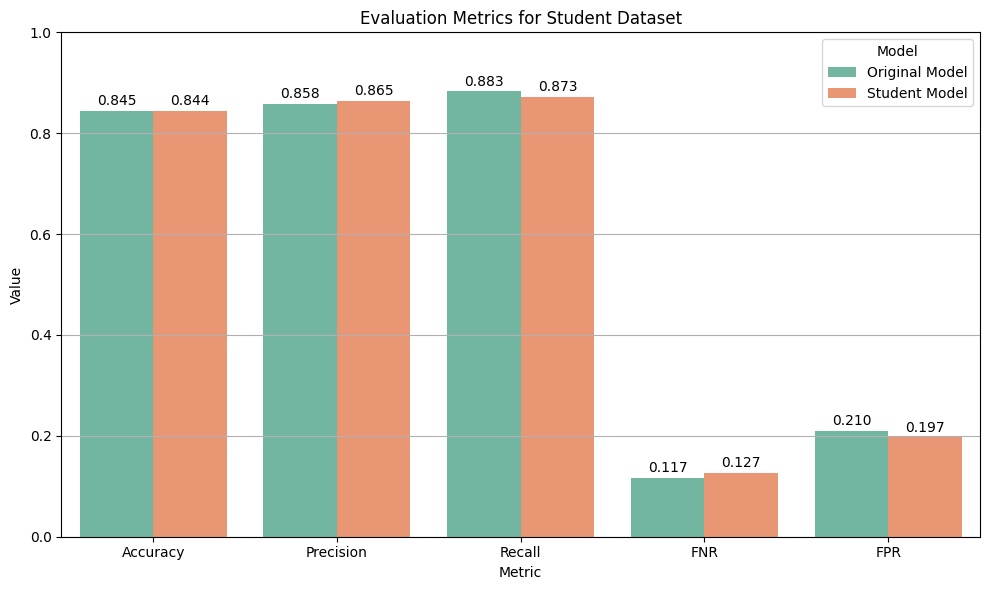
\includegraphics[width=\linewidth]{figures/orig_vs_stu.png} 
    \end{minipage}
    \hfill
   \begin{minipage}{0.49\textwidth}
        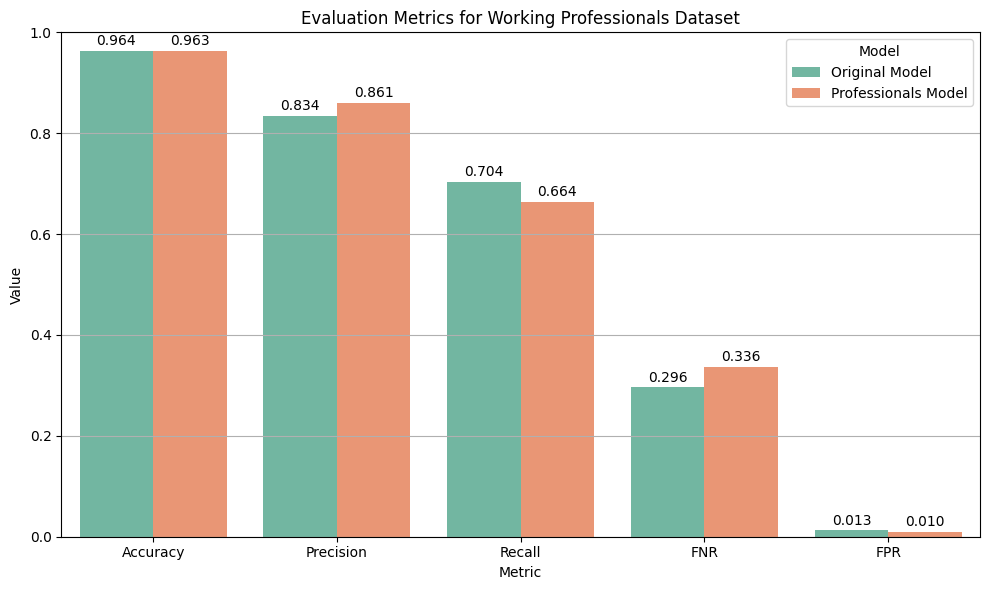
\includegraphics[width=\linewidth]{figures/orig_vs_prof.png} 
    \end{minipage}
    \caption{Metrics Comparison before and after dropping non-relevant features for Students and Working Professionals}
    \label{fig:orig_vs_stu}
\end{figure}

\section{Model Fairness}

To evaluate the fairness of our model, we passed its predictions into \texttt{Fairlearn}’s \texttt{MetricFrame}, using \texttt{Gender} as the sensitive feature. This allowed us to measure not only overall accuracy but also group-specific metrics such as selection rate, false positive rate (FPR), and true positive rate (TPR). These metrics were chosen because they reflect how differently the model behaves across demographic groups in ways that affect real-world outcomes. For example, TPR captures whether the model consistently identifies depression when it is truly present, while FPR reflects the cost of wrongly flagging individuals as depressed. Selection rate offers a lens into how often each group is predicted as positive, regardless of correctness—highlighting disparities in model attention or prioritization. These group-wise metrics provide a more granular understanding of equity than accuracy alone, especially in high-stakes contexts like mental health screening. Contrary to our initial expectations, the model exhibited minimal disparity across gender groups.

\begin{figure}[h]
    \centering
    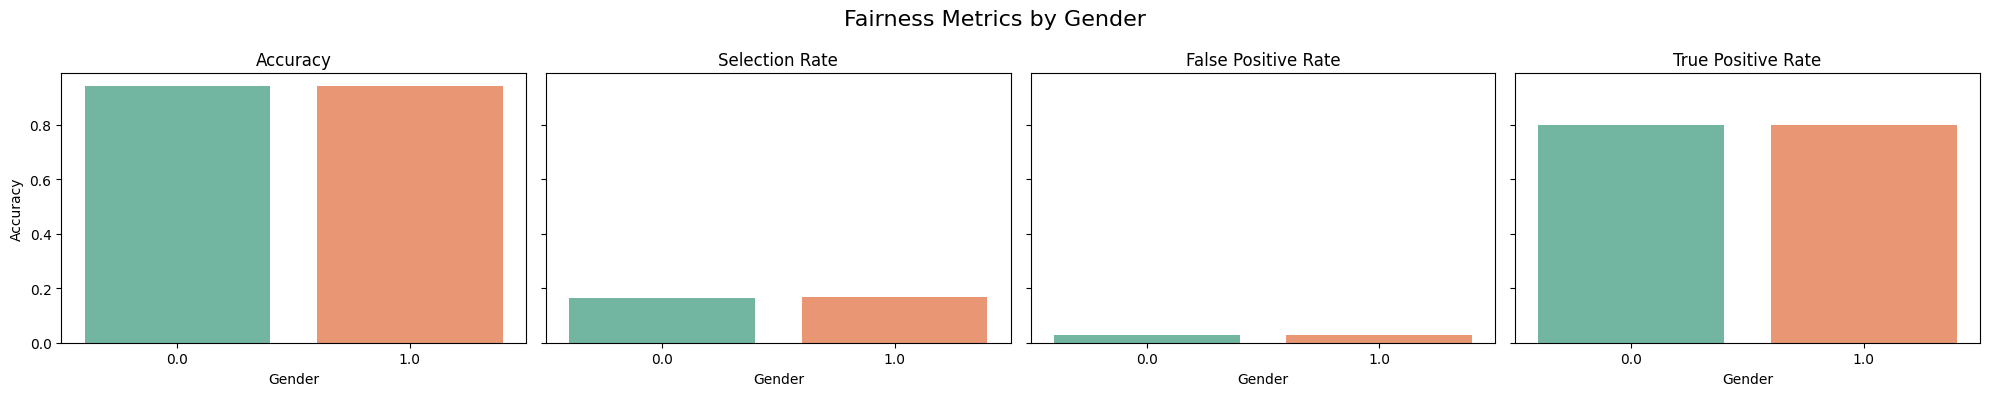
\includegraphics[width=\linewidth]{figures/mf_gender.png}
    \caption{Fairness metrics of the model, with Gender as the sensitive feature.}
    \label{fig:mf_gender}
\end{figure}

As shown in Figure~\ref{fig:mf_gender}, both male and female groups achieve comparable accuracy, selection rate, and error rates. These results suggest that the model is \textit{not} exhibiting strong gender-based bias in its predictions, despite broader societal patterns that might suggest otherwise.

To further validate this finding, we examined fairness across subgroups defined by both \texttt{Gender} and employment status (student or working professional). Once again, we observed no meaningful disparities, as illustrated in Figure~\ref{fig:gender_stu_prof}.

\begin{figure}[h]
    \centering
    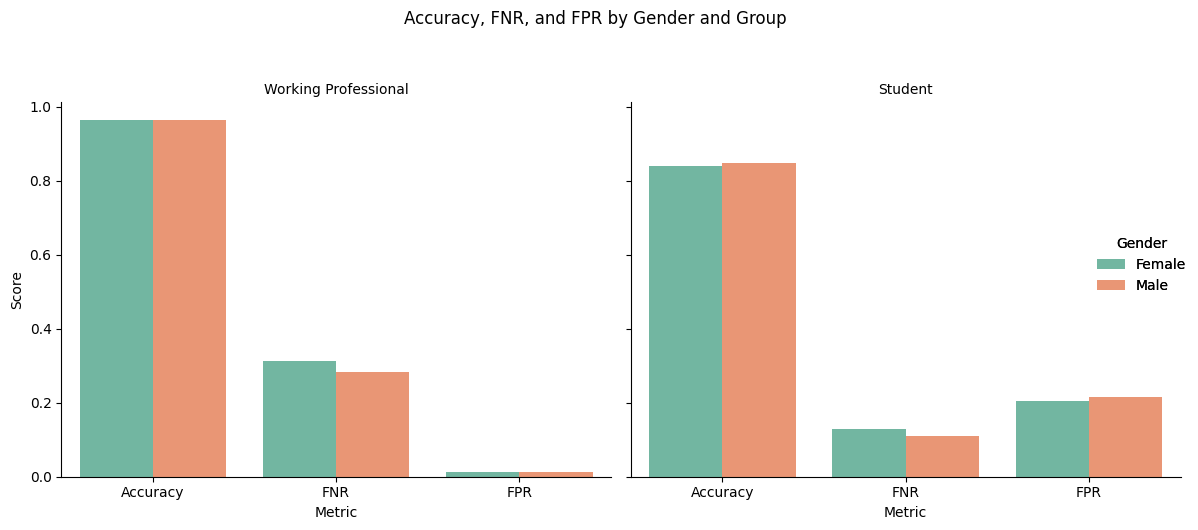
\includegraphics[width=\linewidth]{figures/gender_stu_prof.png}
    \caption{Fairness metrics of the model across employment subgroups, with Gender as the sensitive feature.}
    \label{fig:gender_stu_prof}
\end{figure}

Given the lack of observed gender disparity, we decided to explore alternative sensitive features. Our choice to use \texttt{Working Professional or Student} status as the next axis of analysis was guided by our initial exploratory data analysis. There, we uncovered a strong relationship between age and depression, with younger individuals — particularly students — exhibiting significantly higher depression rates compared to older working professionals. This demographic divide suggests a plausible source of structural disparity that warrants deeper fairness evaluation. By shifting the sensitive feature to employment status, we aim to capture this potentially meaningful divide and investigate whether the model is disproportionately disadvantaging one group over the other.

We again used \texttt{Fairlearn}'s \texttt{MetricFrame} to compute group-wise metrics, this time stratified by employment status. As shown in Figure~\ref{fig:mf_workingorstudent}, the results suggest a measurable disparity. While working professionals (group label 1) achieve higher overall accuracy, their selection rate is substantially lower. In contrast, students (group label 0) are selected by the model at a much higher rate but also experience a higher false positive rate. Notably, their true positive rate is also significantly higher, which could suggest overprediction of the positive class for this group.

\begin{figure}[h]
    \centering
    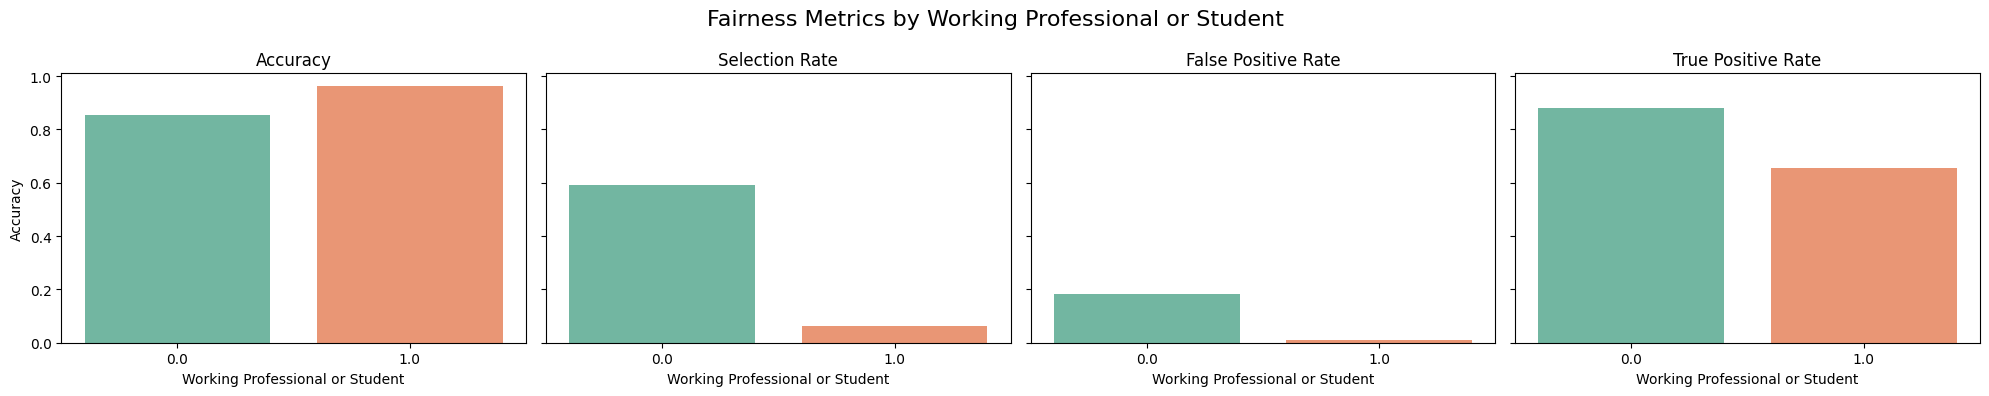
\includegraphics[width=\linewidth]{figures/mf_workingorstudent.png}
    \caption{Fairness metrics of the model, with Working Professional or Student as the sensitive feature.}
    \label{fig:mf_workingorstudent}
\end{figure}

These results suggest that, unlike with gender, the model's predictions vary meaningfully across employment status. This raises potential fairness concerns, particularly in how the model may be over-identifying depression among students while under-identifying it among working professionals. Given the real-world implications of such predictions in mental health interventions, these disparities warrant further investigation and potential mitigation.

To further explore the disparities observed between students and working professionals, we computed and visualized separate confusion matrices for each group. These plots, shown in Figure~\ref{fig:cm_workingorstudent}, provide a more detailed look at how the model behaves in terms of false positives, false negatives, and overall predictive performance for each subgroup.

\begin{figure}[h]
    \centering
    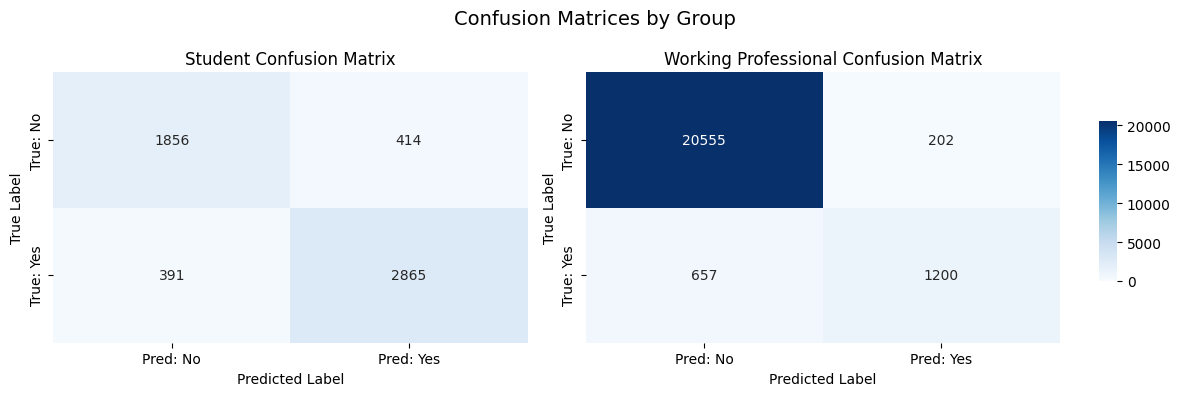
\includegraphics[width=\linewidth]{figures/cm.png}
    \caption{Group-specific confusion matrices with Working Professional or Student as the sensitive feature.}
    \label{fig:cm_workingorstudent}
\end{figure}

Specifically, working professionals not only had a notably higher accuracy ($\sim96\%$) than students ($\sim84\%$), but also higher FNR  ($\sim30\%$), indicating that depressive cases within this group were more likely to go undetected. Additionally, students experienced higher FPR ($\sim21\%$), meaning non-depressive individuals within this subgroup were more likely to be misclassified as depressive. 

In the student group (left panel), we observe a relatively balanced distribution of false positives and false negatives. While the model correctly identifies a large number of depressed students (2,865 true positives), it also generates a considerable number of false positives (414) and false negatives (391). This indicates that the model is relatively sensitive to depression in students, but it also errs in both directions.

By contrast, the confusion matrix for working professionals (right panel) reveals a different pattern. Here, the model shows a strong bias toward predicting the negative class: it identifies a large number of true negatives (20,555) and makes very few false positives (202). However, this comes at the cost of a much higher number of false negatives (657) and fewer true positives (1,200) compared to the student group.

Taken together, these results suggest that the model is more conservative in predicting depression among working professionals. It may be under-identifying true cases in this group, potentially due to differences in underlying feature distributions or label prevalence between students and working professionals. This finding complements the fairness metrics shown earlier and highlights a potential fairness concern: while the model performs well on average, it may systematically fail to detect depression in one group more than the other. This warrants further investigation, especially in high-stakes applications where underdiagnosis can have serious consequences.

To quantify the observed disparities between students and working professionals, we computed group-level disparity scores using a series of metrics provided by the \texttt{fairlearn.metrics} module. These metrics capture the absolute difference in model behavior across the two groups, using \texttt{Working Professional or Student} as the sensitive feature. The results are presented in Table~\ref{tab:ensemble_fairness}.

\begin{table}
\caption{Group-wise performance metrics for the L3 ensemble model using \texttt{Working Professional or Student} as the sensitive feature.}
\label{tab:ensemble_fairness}
\begin{tabular}{lrrrr}
\toprule
 & Accuracy & Selection Rate & True Positive Rate & False Positive Rate \\
\midrule
\textbf{Student (0)} & 0.854300 & 0.603900 & 0.888800 & 0.195200 \\
\textbf{Working Professional (1)} & 0.962000 & 0.062800 & 0.651100 & 0.010200 \\
\bottomrule
\end{tabular}
\end{table}

As shown in the table, the most pronounced disparity appears in the selection rate, with a difference of 0.5314 between groups. This indicates that one group is far more likely to be predicted as positive than the other. Substantial differences are also observed in the true positive rate (0.2337) and false positive rate (0.1726), suggesting that the model’s sensitivity and error patterns vary meaningfully across groups. Even the accuracy difference, which is typically more stable across subpopulations, exceeds 10\%, underscoring that the model’s predictive performance is not uniform between students and working professionals.

Together, these metrics provide strong evidence of group-level disparities in how the model assigns predictions. The magnitude of these differences suggests that additional investigation and potentially mitigation are warranted, especially in applications where equity in prediction outcomes is critical.
 

Again to emphasize, when model was retrained and validated separately for professionals and students (with dropping non-relevant features), these high values of FNR and FPR respectively were maintained (~\ref{fig:orig_vs_stu}). This suggests that the \textit{data} and not just the model architecture drives this disparity. This may be due to the reasons like: (i) Student responses may be more inconsistent or self-reported (and for professionals they might come from clinical diagnoses), leading to noisy ground truth, making the model learn unreliable patterns, causing unstable FPR/FNR tradeoff. Figure~\ref{fig:dep_count_stu} indicates that since ground truth depression for students is much higher than \texttt{Not Depressed}, and even 7-fold higher than Depressed professionals, the model might have overfit, and led to poor generalization. 

\begin{figure}[H]
    \begin{minipage}{0.45\textwidth}
        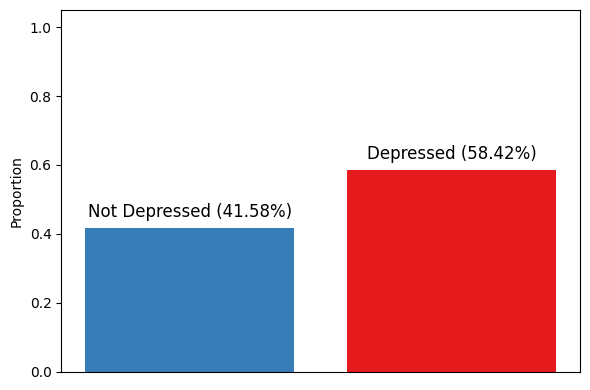
\includegraphics[width=\linewidth]{figures/dep_count_stu.png} 
        \caption{True Counts in Training Data (Students)}
    \label{fig:dep_count_stu}
    \end{minipage}
    \hfill
   \begin{minipage}{0.45\textwidth}
        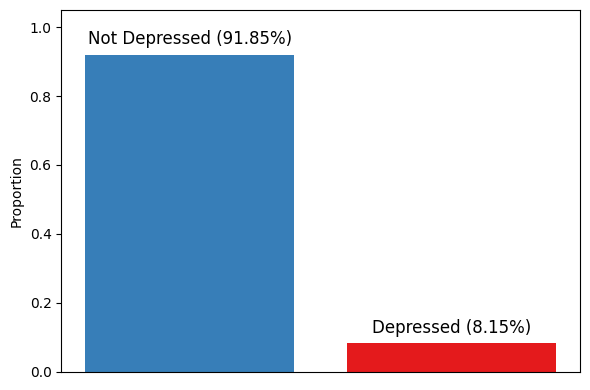
\includegraphics[width=\linewidth]{figures/dep_count_prof.png} 
        \caption{True Counts in Training Data (Working Professionals)}
    \end{minipage}
    \label{fig:dep_count_prof}
\end{figure}

\begin{figure}[H]
    \centering
    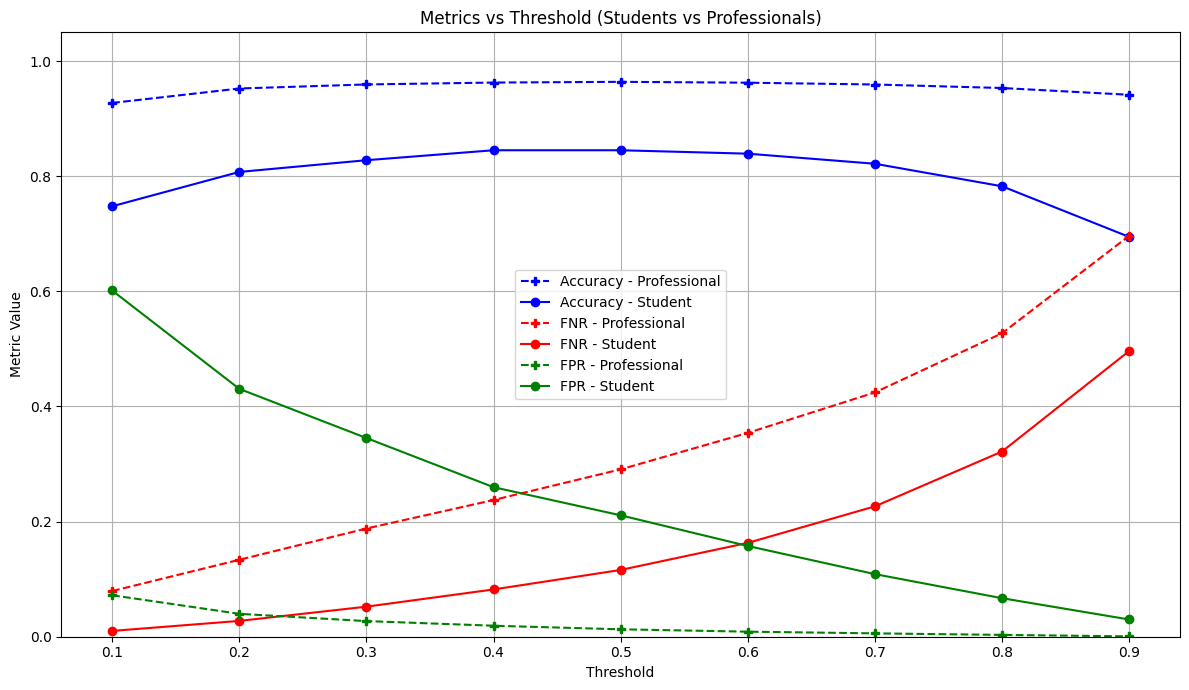
\includegraphics[width=0.7\linewidth]{figures/threshold.png}
    \caption{How metrics change with Classification Threshold}
    \label{fig:threshold}
\end{figure}
(ii) Additionally, the decision threshold (probability less than 0.5 is classified 0, and more than 0.5 is 1) is neither optimized nor group-specific. The same threshold might cause under-detection in professionals (hence high false negative rate) and over-detection in students (high false positive rate). This suggests that overall and group-specific calibration might be necessary. Figure~\ref{fig:threshold} clearly indicates the significant gap in accuracy, FNR, and FPR values between students (bold lines) and working professionals (dotted lines). Though the threshold 0.5 optimizes the gap in accuracy, it doesn't balance the fairness needs of the model. However, an important observation is that even when threshold is modified, there is not much change in accuracy for both the groups, but there can be significant changes in fairness performances, if threshold is optimized. For example, as the threshold increases, false positive rate difference decreases with coming close to 0 at threshold 0.9. 


In acccordance with above observations and to address the fairness disparities observed across employment groups, we applied \texttt{Fairlearn}’s \texttt{ThresholdOptimizer}, a post-processing mitigation technique designed to enforce fairness constraints without retraining the underlying model. In our case, we selected the \texttt{equalized\_odds} constraint, which seeks to equalize both true positive and false positive rates across groups. This choice was motivated by our prior audit, which revealed substantial disparities in sensitivity and error rates between students and working professionals.

Table~\ref{tab:ensemble_fairness_equalized_odds} reports the group-wise performance metrics after threshold optimization. While overall accuracy decreases for the student group, the true positive rates for both groups become closely aligned (0.5992 for students vs. 0.5918 for working professionals), and false positive rates converge as well (0.0370 vs. 0.0385). These results suggest that threshold optimization effectively reduces disparity in model behavior across groups, trading off a modest reduction in predictive performance for improved fairness in classification outcomes.

\begin{table}[H]
\caption{Post-mitigation fairness metrics for the L3 ensemble using \texttt{Working Professional or Student} as the sensitive feature, optimized for equalized odds.}
\label{tab:ensemble_fairness_equalized_odds}
\begin{tabular}{lrrrr}
\toprule
& Accuracy & Selection Rate & True Positive Rate & False Positive Rate \\
\midrule
\textbf{Student (0)} & 0.748600 & 0.368300 & 0.599200 & 0.037000 \\
\textbf{Working Professional (1)} & 0.931100 & 0.084000 & 0.591800 & 0.038500 \\
\bottomrule
\end{tabular}
\end{table}

\begin{figure}[H]
\centering
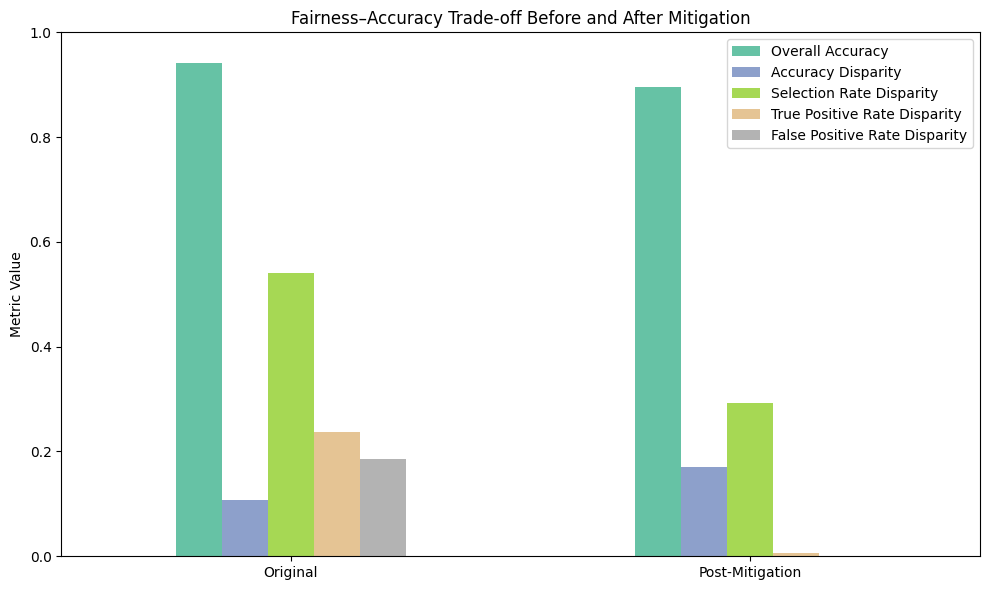
\includegraphics[width=0.6\linewidth]{figures/fairness_tradeoff.png}
\caption{Fairness–accuracy trade-off before and after applying threshold optimization for equalized odds.}
\label{fig:fairness_tradeoff}
\end{figure}
To visualize this trade-off, we compare the original ensemble model and the mitigated version across key fairness and accuracy metrics. As shown in Figure~\ref{fig:fairness_tradeoff}, threshold optimization leads to a small reduction in overall accuracy (from 94\% to 90\%) but results in substantial improvements in fairness: disparities in true and false positive rates nearly vanish, and selection rate disparity decreases by over 40 percentage points. These shifts illustrate the practical cost of enforcing group fairness and highlight the importance of balancing equity and performance in sensitive applications like mental health screening.




\section{Prediction Interpretation}
To better understand how our ensemble model makes predictions—and whether those decisions align with human expectations—we applied LIME (Local Interpretable Model-Agnostic Explanations) \parencite{ribeiro2016why}. LIME explains individual predictions by locally approximating the model with an interpretable surrogate, such as a linear model. However, our final L3 ensemble combines two second-level learners: \texttt{l2-ensemble-lr} (logistic regression) and \texttt{l2-ensemble-ridge} (ridge regression), using a weighted average of their predicted probabilities. While logistic regression exposes the \texttt{predict\_proba} interface needed for LIME, ridge regression does not natively provide probabilistic outputs. Consequently, for interpretability purposes, we restricted LIME analysis to the logistic regression component of the ensemble.

This choice introduces an important caveat: as shown in Figure~\ref{fig:l3_weights}, the final ensemble assigns only \textbf{1.4\%} of the total weight to the logistic regression model, while the ridge regression component dominates with 98.6\%. Therefore, while LIME offers useful intuition into local feature contributions under a linear model, the resulting explanations must be interpreted with caution. They reflect the behavior of a minor contributor to the ensemble, and thus do not fully represent the decision logic of the final model.

\begin{figure}[h]
\centering
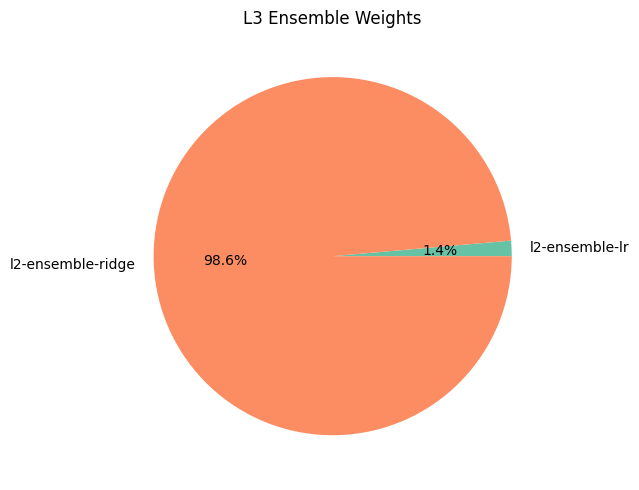
\includegraphics[width=0.4\linewidth]{figures/l2_weights.png}
\caption{L3 ensemble weights assigned to the second-level models. The final prediction is heavily dominated by \texttt{l2-ensemble-ridge}.}
\label{fig:l3_weights}
\end{figure}

Despite this limitation, LIME still provides a transparent lens into how one interpretable component processes the data, and allows us to inspect patterns of misclassification and borderline decisions in a structured way.

We used LIME to analyze three representative validation cases: a misclassified working professional, a misclassified student, and an uncertain but correct prediction. These examples were selected to probe potential group-specific failure modes and examine the model’s behavior near the decision boundary.

\begin{figure}[H]
\centering
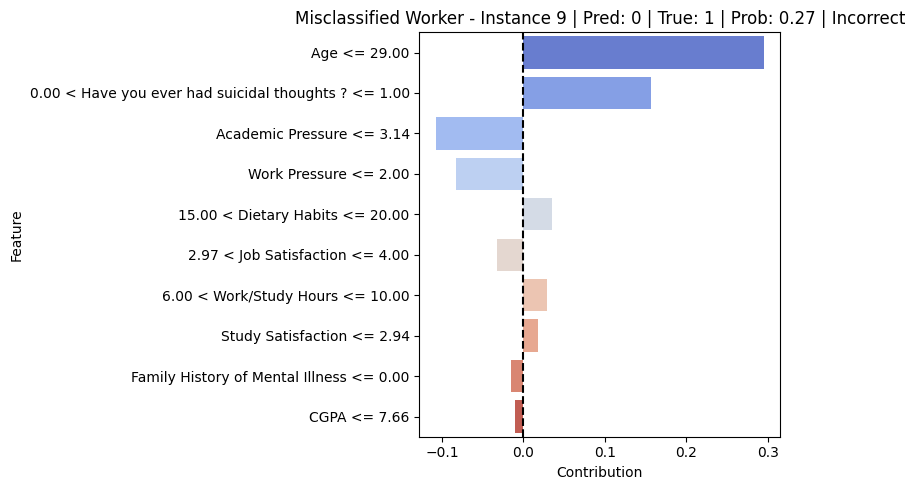
\includegraphics[width=0.9\linewidth]{figures/lime_mis_prof.png}
\caption{LIME explanation for a misclassified working professional (true: depressed, predicted: not depressed). Blue bars indicate features contributing to the negative class (“No”), red bars indicate features contributing to the positive class (“Yes”).}
\label{fig:lime_mis_prof}
\end{figure}

In the first example~\ref{fig:lime_mis_prof}, a working professional was incorrectly classified as not depressed despite self-reporting suicidal ideation and experiencing work pressure. The predicted probability was just 27\%. LIME revealed that older age and low work pressure were dominant negative contributors, outweighing more concerning signals. This case illustrates how the model may be biased toward under-identifying depression among working professionals when protective features are present, even alongside serious risk indicators.


In the second case~\ref{fig:lime_mis_student}, a student was incorrectly classified as depressed, with a predicted probability of 64\%. While this individual showed low financial stress and no family history of mental illness, the model was strongly influenced by age, suicidal ideation, and academic pressure, factors it learned to associate with depression in younger populations. Although understandable, this case demonstrates how the model may over-identify depression among students, consistent with the earlier finding of selection rate disparity by employment group.

\begin{figure}[h]
\centering
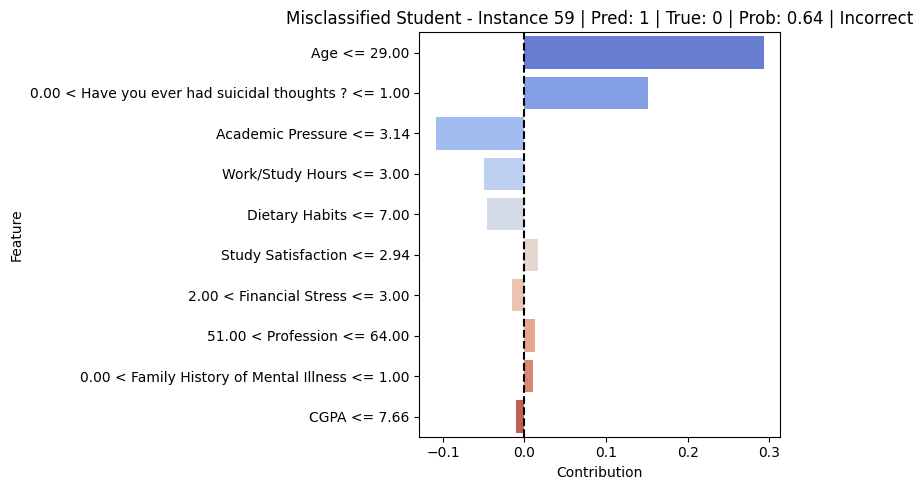
\includegraphics[width=0.8\linewidth]{figures/lime_mis_student.png}
\caption{LIME explanation for a misclassified student (true: not depressed, predicted: depressed).}
\label{fig:lime_mis_student}
\end{figure}

Lastly~\ref{fig:lime_uncertain}, we examined a borderline case with a correct prediction. Here, the model output a probability of 50\% for depression, ultimately predicting the correct label. No single feature dominated the explanation; instead, moderate academic pressure and financial stress were offset by the absence of suicidal thoughts. This example highlights the model’s capacity to handle ambiguity by balancing weak signals, an encouraging sign, though such behavior may also be fragile.

\begin{figure}[h]
\centering
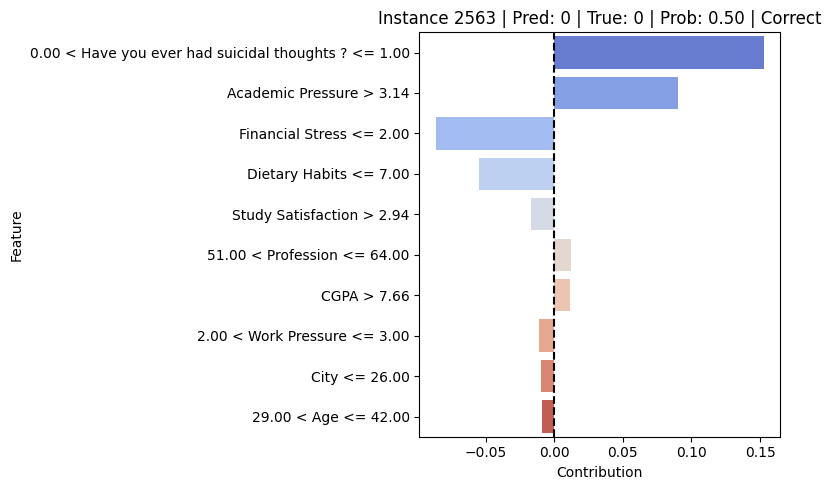
\includegraphics[width=0.75\linewidth]{figures/lime_uncertain.png}
\caption{LIME explanation for a correct but uncertain prediction (true: not depressed, predicted: not depressed, probability: 50\%).}
\label{fig:lime_uncertain}
\end{figure}

These local explanations lend transparency to model behavior, reinforce the fairness concerns raised earlier, and offer valuable guidance for future model debugging and refinement.

